%----------------- KAPITEL : BEISPIELE  ----------------- %	
\chapter{Beispiele}
\label{cha:beispiele}
	Dieses Kapitel soll viele alltaegliche Beispiele\footnote{Fussnote} abdecken um einen {\LaTeX} Dokument zu setzen

		\section{Schriftarten}
		\label{sec:schriftarten} 
			\begin{itemize}
				\item Kursiv: \emph{Das ist ein Beispiel}
				\item Unterstreichen: \underline{Das ist ein Beispiel}
				\item Fettschrift: \textbf{Das ist ein Beispiel}
				\begin{itemize} 
					\item Kombination aus dreien: \underline{\textbf{\emph{Das ist ein Beispiel}}}						\end{itemize} 
				\item Serifen: \textsf{Das ist ein Beispiel}
				\item Schreibmaschinen Schrift: \texttt{Das ist ein Beispiel}
				\item Kleine Grossbuchstassen: \textsc{Das ist ein Beispiel}
				\item Ausfuehrungszeichen: ``Das ist ein Beispiel''
				\item asld
			\end{itemize}
			
		
			\subsection{Symbole}
				\begin{enumerate}
				\item Deutsche Umlaute: "A, "O, "U, "a, "o, "u, "s
				\item Sammlung von Sonderzeichen \url{http://de.wikibooks.org/wiki/LaTeX-Kompendium:_Sonderzeichen}
				\end{enumerate}
				

	\section{Abbildungen}
		Wie folgt bindet man Abbildungen ein:
		% Beispiel für Bildintegration
		\begin{figure}[htb]
		 \centering
		 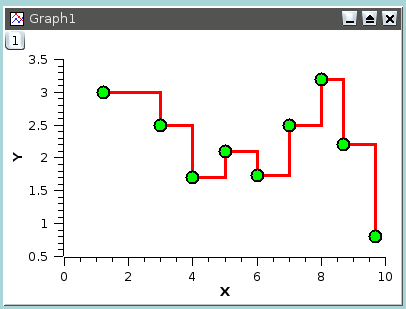
\includegraphics[width=0.4\textwidth,angle=0]{media/beispiel}
 		\caption{Beispiel Bild; Quelle ist png}
		\label{fig:beispiel}
		\end{figure}
	
	\section{Tabellen}
			Lorem ipsum dolor sit amet, consetetur sadipscing elitr, sed diam nonumy eirmod tempor invidunt ut labore et dolore magna aliquyam erat, sed diam voluptua. At vero eos et accusam et justo duo dolores et ea rebum. Stet clita kasd gubergren.

		\begin{center}
			\begin{tabular}{lcrc} \toprule
			Stadium & Substratfreie Kontrolle  & \multicolumn{2}{c}{Probenansatz} \\\cmidrule(rl){3-4}
			 & Farbe & Farbe & Bewertung \\\midrule
			Alpha1 & farblos & braun & +++ \\
			Beta2 & farblos & farblos & - \\\bottomrule 
			 \end{tabular}
		 \end{center}
		 
		2. Beispiel \\
		\begin{table}[h]
		\centering	 
		 	\begin{tabular}{|l|l|c|}
			\hline
			\textsc{Rang} & \textsc{Name} & \textsc{Rating}\\
			\hline
			\hline
			1 & Garry Kasparov & 2817\\
			2 & Viswanathan Anand & 2774\\
			3 & Wladimir Kramnik & 2764\\
			\hline
			\end{tabular}
		\caption{Beispiel Beschriftung einer Tabelle}
		\label{tab:beispiel}
		\end{table}
		
		


	\section{Verweise}
		Hier werden Verweise auf verschiedene Elemente erstellt \cite{lin1973}
		\subsection{Pageref und Ref} 
			Diese Textstelle ist sehr interessant.\label{interessant} \\				
			Hier wird auf die Textstelle~\ref{interessant} verwiesen, \\
			die sich auf der Seite~\pageref{interessant} befindet.\\[20pt] 
			Verweis auf Listing \ref{lst:javaBsp} auf Seite \pageref{lst:javaBsp} \\
			Verweis auf Abbildung \ref{fig:beispiel} auf Seite \pageref{fig:beispiel} \\
			Verweis auf Tabelle \ref{tab:beispiel} auf Seite \pageref{tab:beispiel}
			
	\section{Listing}
		\lstset{language=java}
		\begin{lstlisting}[frame=hl, caption={Das Listing zeigt Java Quellcode} ,backgroundcolor=\color{gray}, label={lst:javaBsp}]
/* Java Hallo World Beispiel */

public class HelloWorld {
    public static void main(String[] args) {
        System.out.println("Hello, World");
    }
}
		\end{lstlisting} 
		
	
\nocite{wiki:xxx}